%%%%%%%%%%%%%%%%%%%%%%%%%%%%%%%%%%%%%%%%%
% Beamer Presentation
% LaTeX Template
% Version 1.0 (10/11/12)
%
% This template has been downloaded from:
% http://www.LaTeXTemplates.com
%
% License:
% CC BY-NC-SA 3.0 (http://creativecommons.org/licenses/by-nc-sa/3.0/)
%
%%%%%%%%%%%%%%%%%%%%%%%%%%%%%%%%%%%%%%%%%

%----------------------------------------------------------------------------------------
%	PACKAGES AND THEMES
%----------------------------------------------------------------------------------------

\documentclass{beamer}

\mode<presentation> {

% The Beamer class comes with a number of default slide themes
% which change the colors and layouts of slides. Below this is a list
% of all the themes, uncomment each in turn to see what they look like.

%\usetheme{default}
%\usetheme{AnnArbor}
%\usetheme{Antibes}
%\usetheme{Bergen}
%\usetheme{Berkeley}
%\usetheme{Berlin}
%\usetheme{Boadilla}
\usetheme{CambridgeUS}
%\usetheme{Copenhagen}
%\usetheme{Darmstadt}
%\usetheme{Dresden}
%\usetheme{Frankfurt}
%\usetheme{Goettingen}
%\usetheme{Hannover}
%\usetheme{Ilmenau}
%\usetheme{JuanLesPins}
%\usetheme{Luebeck}
%\usetheme{Madrid}
%\usetheme{Malmoe}
%\usetheme{Marburg}
%\usetheme{Montpellier}
%\usetheme{PaloAlto}
%\usetheme{Pittsburgh}
%\usetheme{Rochester}
%\usetheme{Singapore}
%\usetheme{Szeged}
%\usetheme{Warsaw}

% As well as themes, the Beamer class has a number of color themes
% for any slide theme. Uncomment each of these in turn to see how it
% changes the colors of your current slide theme.

%\usecolortheme{albatross}
%\usecolortheme{beaver}
%\usecolortheme{beetle}
%\usecolortheme{crane}
%\usecolortheme{dolphin}
%\usecolortheme{dove}
%\usecolortheme{fly}
%\usecolortheme{lily}
%\usecolortheme{orchid}
%\usecolortheme{rose}
%\usecolortheme{seagull}
%\usecolortheme{seahorse}
%\usecolortheme{whale}
%\usecolortheme{wolverine}

%\setbeamertemplate{footline} % To remove the footer line in all slides uncomment this line
%\setbeamertemplate{footline}[page number] % To replace the footer line in all slides with a simple slide count uncomment this line

%\setbeamertemplate{navigation symbols}{} % To remove the navigation symbols from the bottom of all slides uncomment this line
}

\usepackage{graphicx} % Allows including images
\usepackage{booktabs} % Allows the use of \toprule, \midrule and \bottomrule in tables
\usepackage{amsmath}
\usepackage{amssymb}
\usepackage[author-year]{amsrefs}


%----------------------------------------------------------------------------------------
%	TITLE PAGE
%----------------------------------------------------------------------------------------

\title[Newton Bases for Interpolation]{Kernel Newton Bases for Interpolation} % The short title appears at the bottom of every slide, the full title is only on the title page

\author{Tim McCollam} % Your name
\institute[IIT] % Your institution as it will appear on the bottom of every slide, may be shorthand to save space
{
Illinois Institute of Technology \\ % Your institution for the title page
\medskip
\textit{tmccolla@hawk.iit.edu} % Your email address
}
\date{\today} % Date, can be changed to a custom date

\begin{document}

\begin{frame}
\titlepage % Print the title page as the first slide
\end{frame}

%----------------------------------------------------------------------------------------
%	PRESENTATION SLIDES
%----------------------------------------------------------------------------------------


\begin{frame}
\frametitle{Introduction}
\begin{itemize}
\item Standard interpolation: given a set of data $f(x_i)=\{x_1, x_2, ... , x_n\}$, find a function $\tilde{f}(x)$ that exactly fits all of these points.
\item We assume that $\tilde{f}(x)$ is a linear combination of a data-dependent basis. 
\begin{itemize}
\item i.e. $\tilde{f}(x) = \sum\limits^{n}_{k=1}c_{k}K_{k}(x)$ which leads to the equation $\mathsf{K}\textbf{c}=\textbf{y}$ for which we need to solve for $\textbf{c}$.
\end{itemize}
\item So, we need to choose an appropriate $\mathsf{K}$ (i.e. an appropriate basis) which is invertable and does not have conditioning issues.
\end{itemize}
\end{frame}


\begin{frame}
\frametitle{Introduction}
\begin{itemize}
\item A common basis used is the Kernel Basis: use radial basis functions such as the Gaussian $K(x_i,x_j)=e^{\epsilon^2\|x_i-x_j\|^2}$ to construct the matrix.
\begin{itemize}
\item $\mathsf{K}=(K(x_i,x_j))^{n}_{i,j=1}$
\end{itemize}
\item According to \ocite{MulSch09a} and \ocite{PazSch11a}, there exists a basis called the Newton Basis which has better conditioning than the typical Kernel Basis.
\end{itemize}
\end{frame}


\begin{frame}
\frametitle{Newton Basis}
\begin{itemize}
\item We want basis functions $v$ such that
	\begin{itemize}
	\item $v_j(x_i)=0$ for $i<j$
	\item $v_j(x_j)=1$
	\item span$\{v_1, ... , v_m\}=$ span$\{k_1, ... k_n\}$ where the $k_i$'s are the standard Kernel Basis.
	\end{itemize}
\item We calculate the Newton Matrix $\mathsf{V}$ with: 
\begin{itemize}
\item $\beta_{ij}=K(x_i,x_j)-\sum\limits^{i-1}_{k=0}{\beta_{jk}v_{k}(x_i)}$ for $i\leq j$
\item  $\beta_{ij}= 0$ for $i>j$
\end{itemize}
\end{itemize}
\end{frame}

\begin{frame}
\frametitle{Newton Basis}
\begin{itemize}
\item We also add the ability to exactly interpolate linear equations by adding $\alpha_1+\alpha_2 x$ to $\tilde{f}(x)$. This results in the matrix
$\tilde{\mathsf{V}}=$$\begin{bmatrix}
\mathsf{V}&\mathsf{P}^T\\\mathsf{P}&0
\end{bmatrix}$
where
$\mathsf{P}=\begin{bmatrix}
1&...&1\\
x_1 &... &x_n
\end{bmatrix}$
\item We then adjust the original equation that needs to be solved to\\ $\tilde{\mathsf{V}}$
$\begin{bmatrix}
\mathbf{c}\\
\alpha_1\\
\alpha_2 x
\end{bmatrix}=\begin{bmatrix}
\mathbf{y}\\
\mathbf{0}
\end{bmatrix}$ \\
and we add the conditions that \\$\sum\limits^n_{k=1}c_k = 0$ and \\$\sum\limits^n_{k=1}c_{k}x_k = 0$
\end{itemize}
\nocite{fass07}
\end{frame}

\begin{frame}
\frametitle{Condition Numbers}
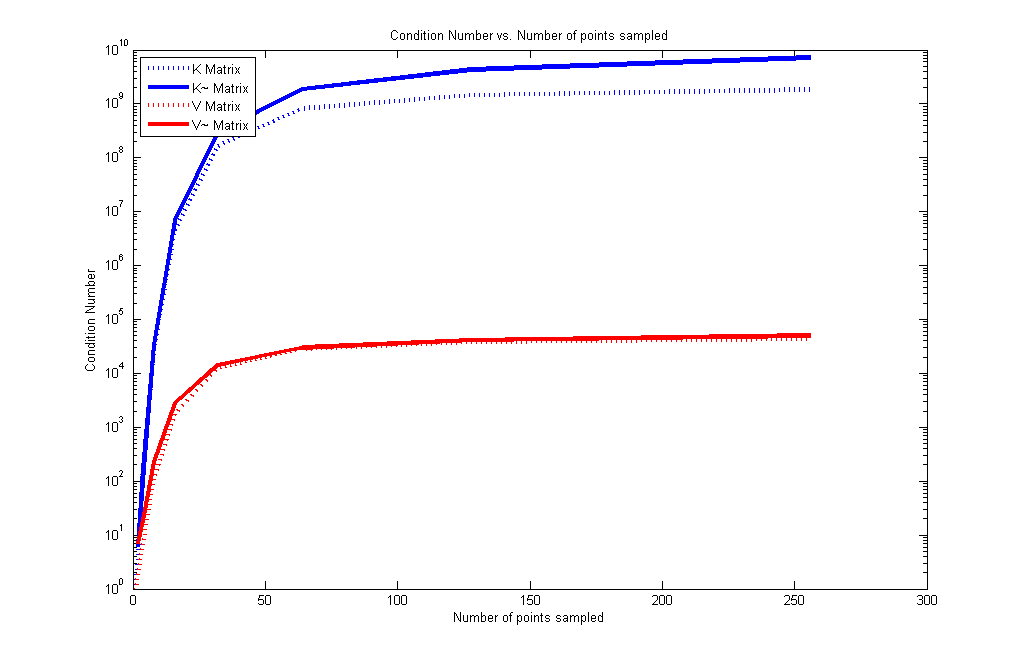
\includegraphics[scale = .45]{condNum}
\end{frame}

\begin{frame}
\frametitle{Interpolation}
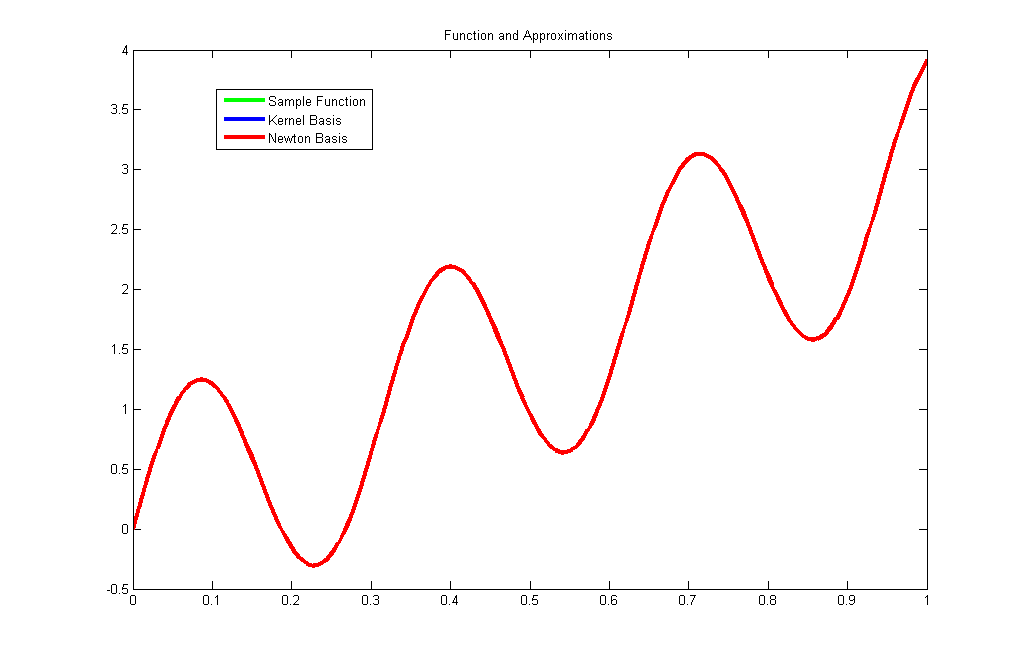
\includegraphics[scale = .45]{functionAppx}
%put interpolation graph here
\end{frame}

\begin{frame}
\frametitle{Error Estimation}
\begin{itemize}
\item By the method of power functions, $\|f(x)-\tilde{f}(x)\| \leq \|f\|\sqrt{K(x, x)-\mathbf{k}^T(x)\mathsf{K}^{-1}\mathbf{k}(x)}$
\item Similarly, for the Newton Basis  $\|f(x)-\tilde{f}(x)\| \leq \|f\|\sqrt{K(x, x)-\mathbf{v}^T(x)\mathsf{V}^{-1}\mathbf{v}(x)}$
\item \cite{fass07}
\end{itemize}
\end{frame}

\begin{frame}
\frametitle{Error}
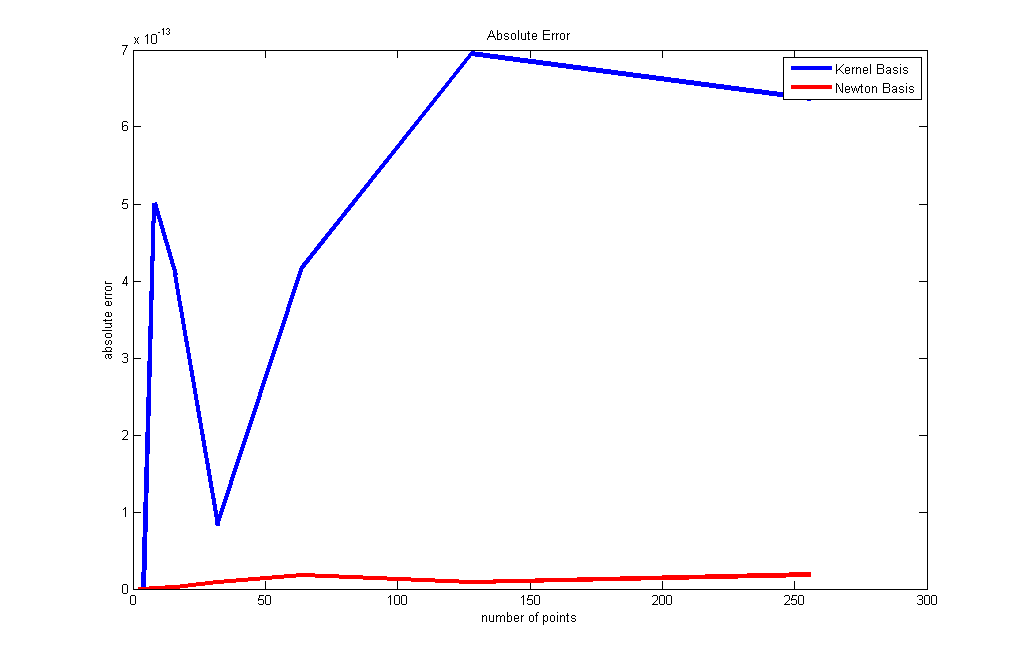
\includegraphics[scale =.45]{functionError}
%put error graph here
\end{frame}

\begin{frame}\frametitle{References}
\bibliography{FJH22,FJHown22}
\end{frame}

%------------------------------------------------

\begin{frame}
\Huge{\centerline{Thank You!}}
\end{frame}

%----------------------------------------------------------------------------------------

\end{document} 